\chapter{Anexos}

\section{Código Fuente Octave}
\label{sec.ej1:anexo_octave}

A continuación se adjunta el script utilizado para la generación de los diagramas de Bode y el análisis de la función
de transferencia. Se utilizó la biblioteca \texttt{bodas} \cite{bodas} para la representación gráfica.

\lstinputlisting[style=octave, caption={Script de Octave para el Ejercicio 1.}]{sources/ej1.m}

\section{Trabajo en Papel}
\label{sec.ej1:anexo_papel}

Se adjuntan las hojas del desarrollo analítico realizado manualmente durante la resolución del ejercicio.

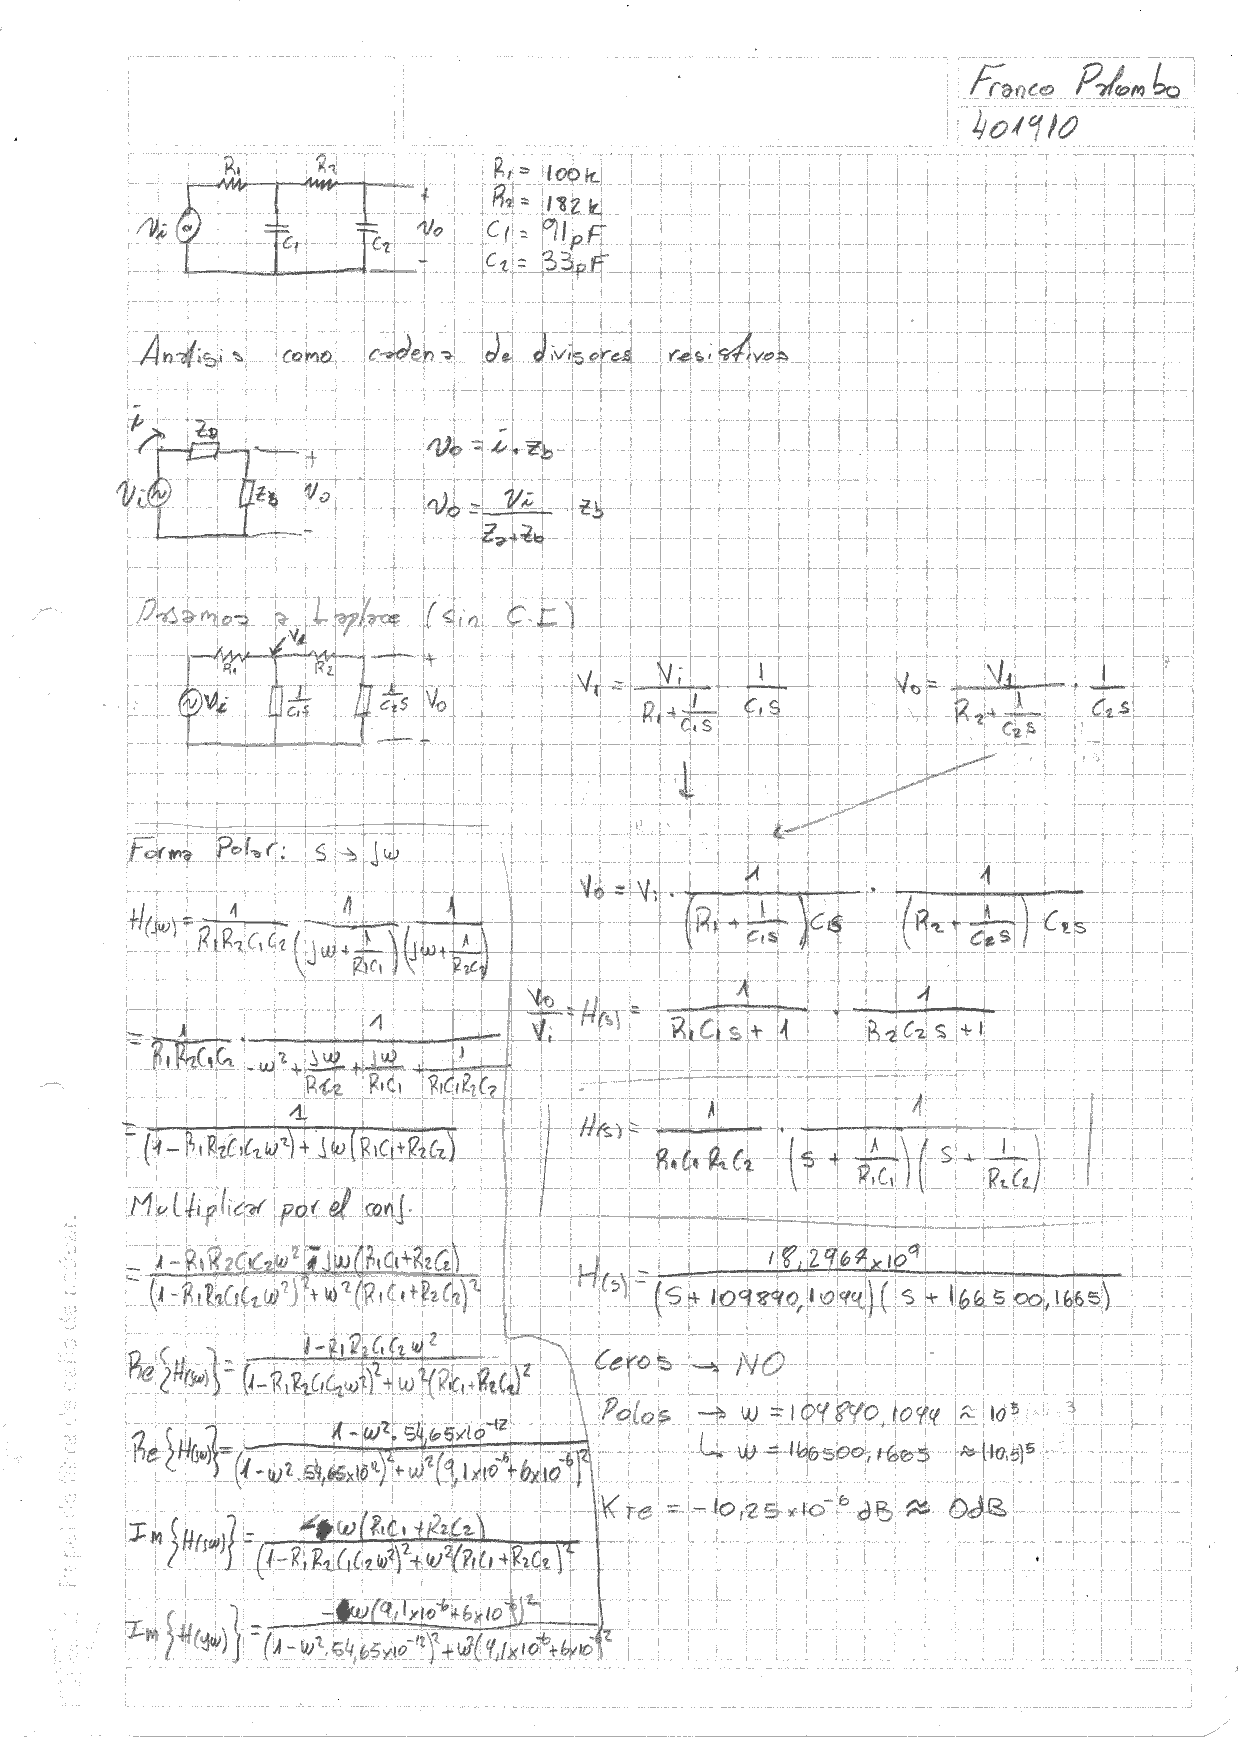
\includepdf[pages=-]{sources/tdc2_tp1_ej1_res.pdf}
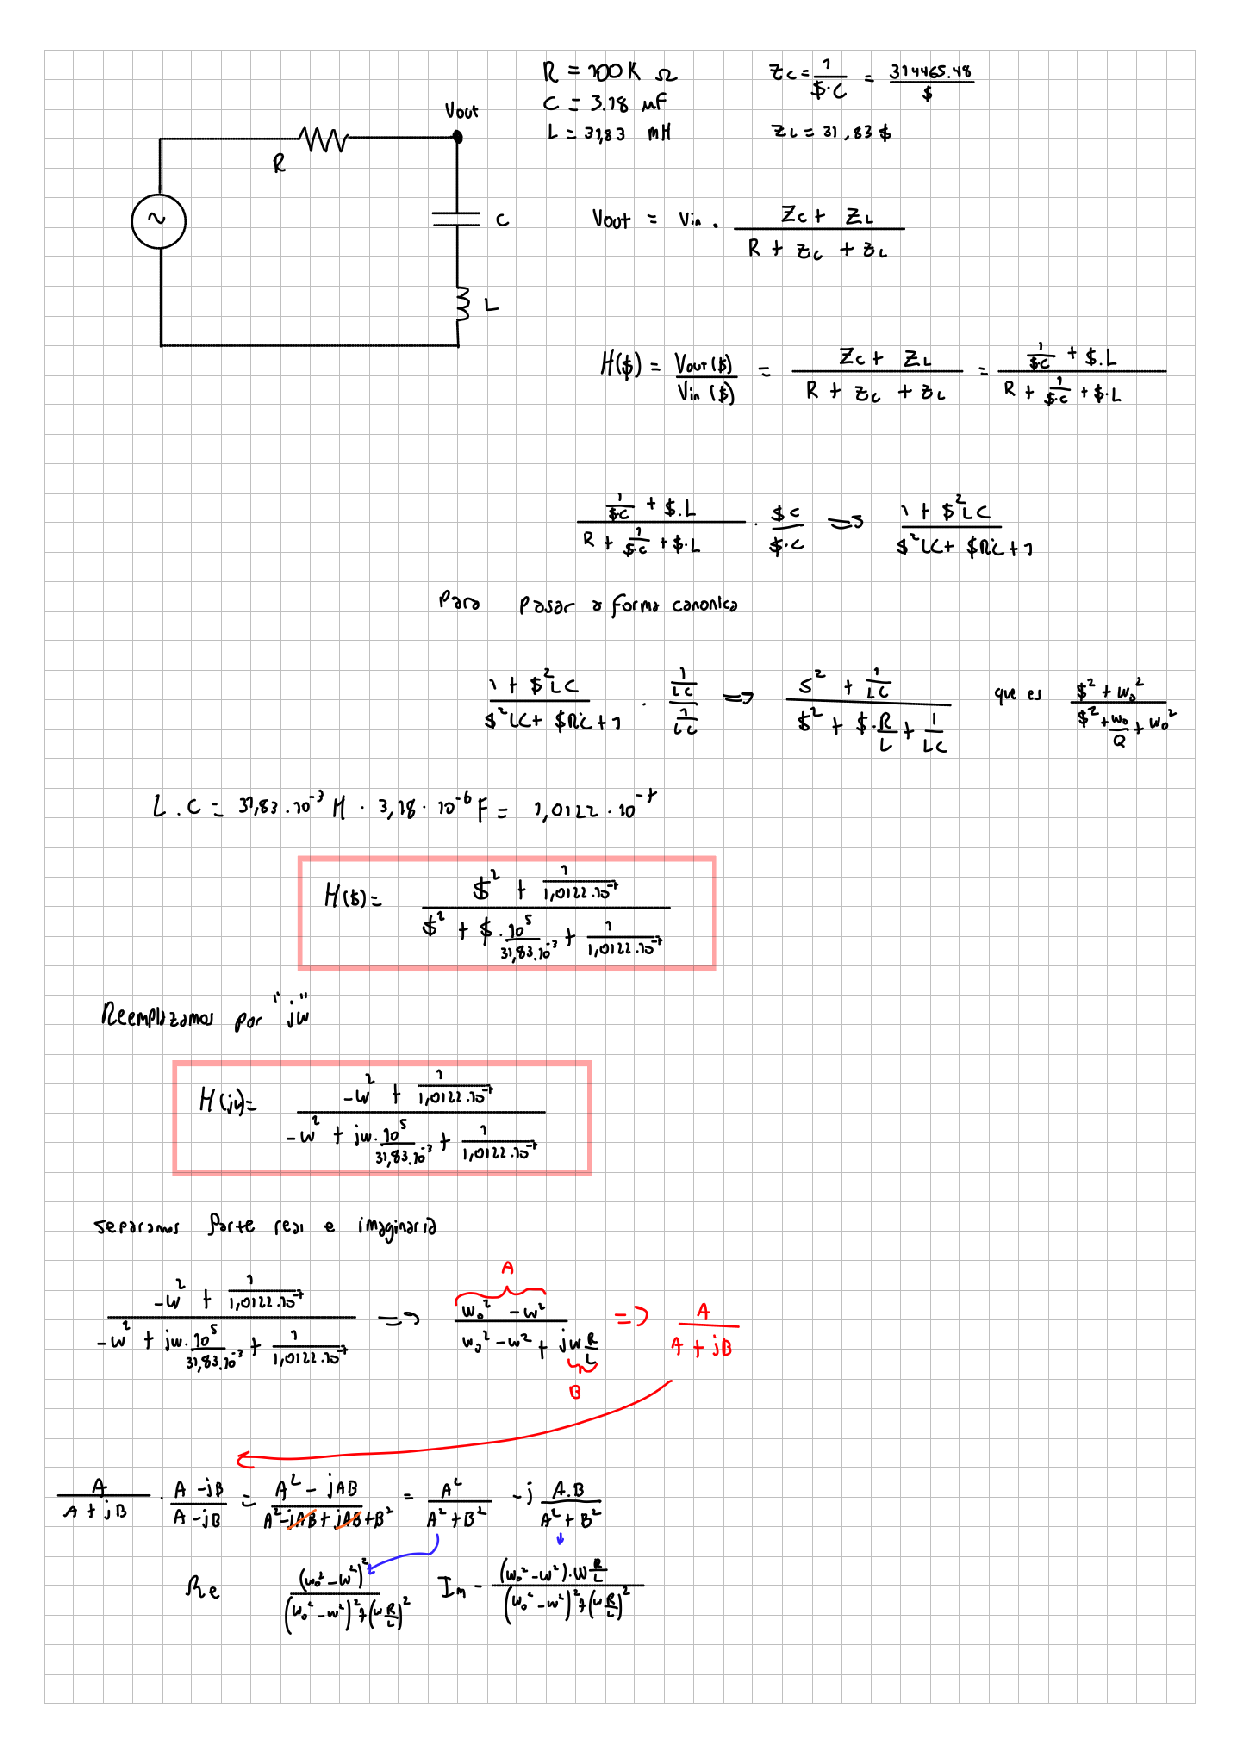
\includepdf[pages=-]{sources/Ej2_tp1_resolucion.pdf}
